\chapter{PLANTEAMIENTO DEL PROBLEMA}
\section{Descripción de la Realidad Problemática}

Desde inicios de la historia, las enfermedades infecciosas hasta crónicas han sido parte de la humanidad y han afectado desde pueblos hasta naciones. No obstante, gracias al avance de la medicina se ha podido comprender muchas de estas enfermedades, logrando mejorar la salud de muchas personas o su completa recuperación. Pero en el mejor de los casos eliminada o controlada por completo, el caso más conocido es la viruela que fue erradicada en 1980 debido a un programa mundial de vacunación. 


\begin{figure}[h]
	\begin{center}
		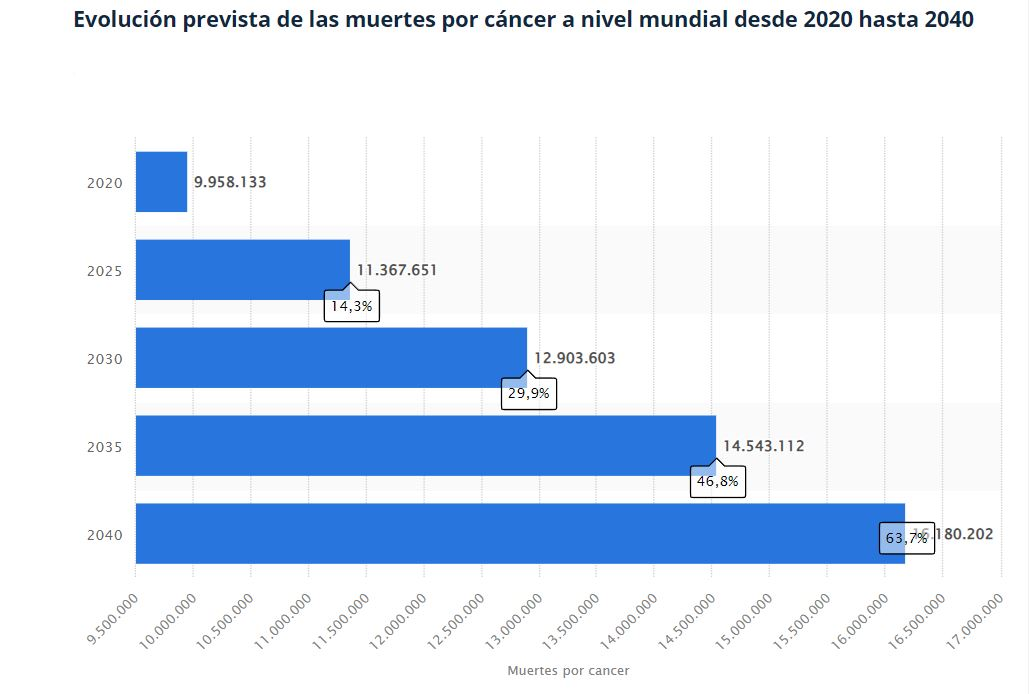
\includegraphics[width=0.75\textwidth]{1/figures/Grafico1DiagnosnitoCancer.JPG}
		\caption{Predicción de número de casos acumulado de cancer a nivel mundial. Fuente: \cite{stadisitc_cancer}}
		\label{1:fig}
	\end{center}
\end{figure}


Sin embargo, una enfermedad que ha afectado durante siglos a la humanidad es el cáncer. Este se caracteriza por su capacidad de alterar el equilibrio de las células del cuerpo humano, provocando un crecimiento anormal y descontrolado de las zonas afectadas a tal grado que puede llegar a invadir otras partes del cuerpo. La Organización mundial de la salud (OMS) afirma que el cáncer es la segunda causa muerte más frecuente en América y una las principales a nivel mundial. En estima que en el año 2022 hubo 20 millones de nuevos casos y 9,7 millones de muertes. Como se pude observar en la figura\ref{1:fig}, según el estudio de Statista publicado en el año 2023 se proyecta que el número de nuevos casos de cáncer crecerá notoriamente en los próximos 20 años.\parencite{OMS_cancer}






Entre los tipos más comunes de cáncer se encuentra el que afecta a la piel el cual se puede contraer a cualquier edad; sin embargo, las personas de mayor riesgo son las que estan expuestos por tiempos prolongados al sol y poseen piel clara. La principal causa es la exposición a la radiación ultravioleta o fuentes artificiales. Según American Cancer Society para el año 2023 morirán aproximadamente que morirán aproximadamente 7,990 personas y aproximadamente aparecerán 97,610 nuevos casos.

Si bien la mayoría de los casos se puede tratar sin complicaciones, existe un porcentaje en el cual puede llegar a ser peligro y potencialmente mortal. Esto principalmente debido a que no es detectado a tiempo o no se cuenta con dermatólogos especializados en esta área.

\begin{figure}[h]
	\begin{center}
		\includegraphics[width=0.5\textwidth]{1/figures/radiación_ultravioleta_peru.png}
		\caption{Pronóstico de radiación UV. Fuente: \cite{SENAMHI_uv}}
		\label{1:fig1}
	\end{center}
\end{figure}



En el caso del Perú, el cáncer de piel está en aumento, especialmente debido a la alta incidencia de radiación ultravioleta (UV) en muchas regiones del país como podemos ver en la figura\ref{1:fig1} el nivel de radiacion ultravioleta el dia 21 de abril del 2024 \parencite{SENAMHI_uv}  y la falta de conciencia sobre la protección solar adecuada. Agregando, la detección temprana y el tratamiento oportuno de esta enfermedad son difíciles por la falta de acceso a servicios de salud especializados en algunas áreas rurales y remotas. Como podemos observar en la siguente figura\ref{1:fig2} La cual nos indica que el 73\%\ de los casos fueron cuando acudieron a un establecimiento de salud en el momento que ya presentaron síntomas muy notorios de cáncer, haciendo evidencia de que el fue diagnosticado de forma tardía. \parencite{cancer_diagnostico}



\begin{figure}[h]
	\begin{center}
		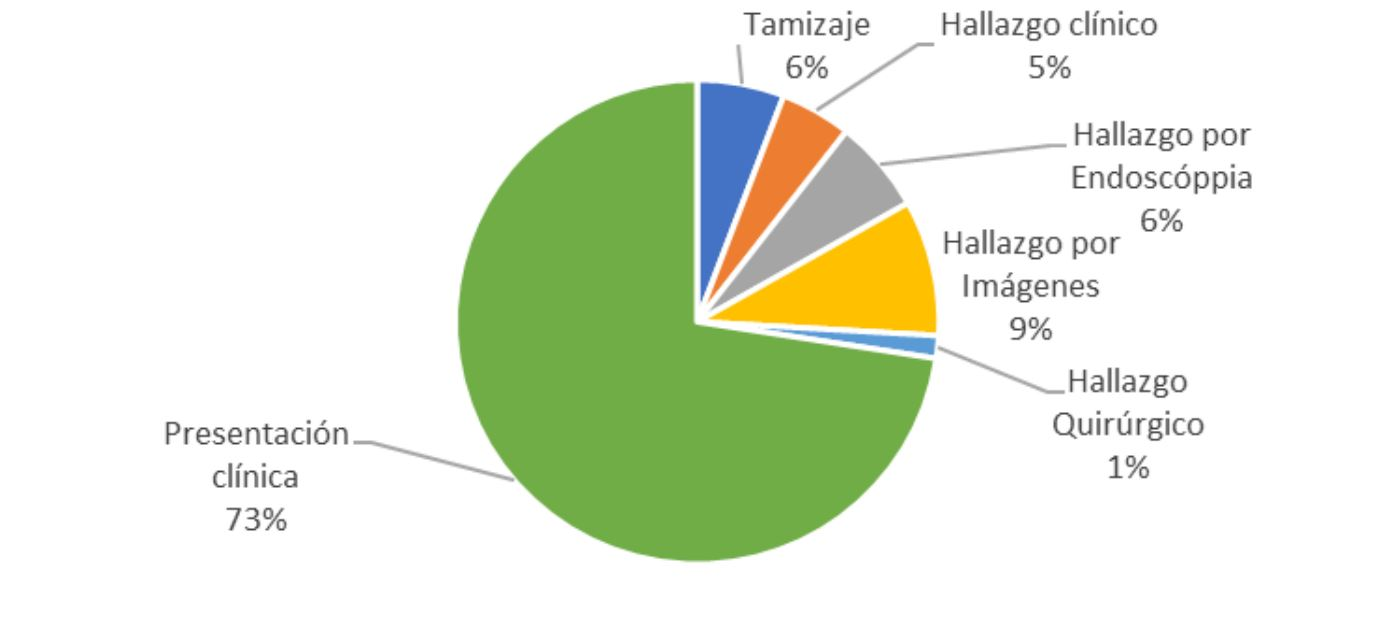
\includegraphics[width=0.8\textwidth]{1/figures/cancer_diagnostico.JPG}
		\caption{Metodo del primer diagnostico DEL CANCER.PERU 2019-2022: \cite{cancer_diagnostico}}
		\label{1:fig2}
	\end{center}
\end{figure}







\section{Formulación del Problema}

Para realizar la formulación de los problemas del presente trabajo, se elaboró un árbol de problemas (Anexo \ref{1:arbolProblema}).

\subsection{Problema General}
\newcommand{\ProblemaGeneral}{¿Cómo dificulta la falta de especialistas dermatológicos en la detección temprana del cáncer de piel en el Perú?
}
\ProblemaGeneral
\subsection{Problemas Espec\'{i}ficos}
\newcommand{\Pbone}{
¿Cuáles son los algoritmos de Deep Learning que pueden clasificar con precisión los melanomas y no melanomas entre pacientes peruanos?
}
\newcommand{\Pbtwo}{
¿Cuál es el desafío principal entre reconocer los tipos de cáncer en los pacientes peruanos?
}
\newcommand{\Pbthree}{
¿Qué tipo de ruido pude haber en las imagenes que dificulté la clasificación de los melanomas y no melanomas entre pacientes peruanos?
}
\newcommand{\Pbfour}{
¿ Qué alternativas se proponen en los trabajos previos para seleccionar características y desarrollar el marco de trabajo de la investigación?
}
\newcommand{\Pbfive}{
¿Cuál es la influencia de las condiciones ambientales y geográficas específicas de Perú en el tratamiento del cáncer de piel?
}

\begin{itemize}
	\item \Pbone
	\item \Pbtwo
	\item \Pbthree
	\item \Pbfour
	\item \Pbfive
\end{itemize}

\section{Objetivos de la Investigación}

Para realizar la formulación de los problemas del presente trabajo, se elaboró un árbol de objetivos (Anexo \ref{1:arbolObjeti}).


\subsection{Objetivo General}
\newcommand{\ObjetivoGeneral}{
Desarrollar un sistema de detección de cáncer de piel mediante el uso de técnicas de Deep Learning y visión por computadora que permita identificar lesiones dermatológicas a partir de imágenes, para realizar una detección temprana.

%%Determinar cuál de las herramientas propuestas en los trabajos previos es la más precisa y confiable en la detección utilizando imágenes dermatoscopias de pacientes peruanos

}
\ObjetivoGeneral
\subsection{Objetivos Espec\'{i}ficos}
\newcommand{\Objone}{
Identificar y comparar los algoritmos de Deep Learning más adecuados para la clasificación de melanomas y no melanomas en imágenes dermatoscópicas de pacientes del Perú.
}
\newcommand{\Objtwo}{
Analizar cómo las características dermatoscópicas únicas en Perú afectan el reconocimiento de melanomas y no melanomas de pacientes del Perú.
}
\newcommand{\Objthree}{
Identificar y evaluar el impacto de estos ruidos en la precisión de la clasificación de melanomas y no melanomas de pacientes del Perú.
}
\newcommand{\Objfour}{
Analizar los diferentes enfoques utilizados en investigaciones anteriores con la finalidad de desarrollar marcos de trabajo efectivos para la clasificación de melanomas y no melanomas de pacientes del Perú.
}
\newcommand{\Objfive}{
Analizar cómo las condiciones ambientales y geográficas pueden afectar los melanomas y no melanomas de pacientes del Perú.
}

\begin{itemize}
	\item {\Objone}
	\item {\Objtwo}
	\item {\Objthree}
	\item {\Objfour}
	\item {\Objfive}
\end{itemize}


\section{Hipótesis}

\subsection{Hipótesis General}
\newcommand{\HipotesisGeneral}{
La aplicación de técnicas de Deep Learning en el análisis de imágenes dermatoscópicas permitirá entrenar un modelo capaz de identificar características específicas asociadas con el cáncer de piel con una precisión igual o superior a la de los dermatólogos especializados, facilitando la detección temprana de esta enfermedad

}
\HipotesisGeneral
\subsection{Hipótesis Específicas}
\newcommand{\Hone}{
	La implementación del algoritmo de Deep Learning adecuado permitirá calcificar con alta precisión los tipos de cáncer de piel melanomas y no melanomas
	
}
\newcommand{\Htwo}{
	Determinar los tipos de características dermatoscopias que afecta el reconocimiento de melanomas y no melanomas de pacientes del Perú.
	
}
\newcommand{\Hthree}{
	Identificar los tipos de ruidos en las imágenes dermatológicas permitirá tener un modelo con mayor precisión
		
}
\newcommand{\Hfour}{
	Análisis de trabajos previos para el desarrollo de métodos efectivos con la finalidad de mejorar la eficiencia de los modelos.
	
}
\newcommand{\Hfive}{
	Influencia de las condiciones ambientales y geográficas influye en el cáncer de tipo melanomas y no melanomas de pacientes del Perú.
}
\begin{itemize}
	\item \Hone
	\item \Htwo
	\item \Hthree
	\item \Hfour
	\item \Hfive
\end{itemize}

\subsection{Matriz de Consistencia}

Esta fue elavorada para la presente investigación en el cual encontrarn los problemas, objetivos e hipótesis descritas anteriormente en el Anexo \ref{1:table}.

%%Los problemas, objetivos e hipótesis descritas anteriormente se encuentran en la Matriz de Consistencia del Anexo \ref{table}. Además, los objetivos específicos se formularon a partir de una lluvia de ideas luego de examinar los objetivos planteados en los antecedentes, cuyo detalle e item de referencia se encuentra en el Anexo \ref{anexo5}.


%A continuación se presenta la matriz de consistencia elaborada para la presente investigación (véase Anexo \ref{1:table}).


\section{Justificación de la Investigación}

\subsection{Teórica}
Este trabajo de investigación se realiza con la finalidad de apoyar la falta de dermatólogos especialistas en ciertas regiones del Perú.

Haciendo uso de tecinas de Deep Learning en el análisis de imágenes dermatológicas puede predecir si un usuario pueda estar desarrollando cáncer de piel y predecir el tipo. 


\subsection{Práctica}
Existen diversas investigaciones donde se realiza pre-diagnosticos o clasificación de que tipo de cáncer de piel se muestra en la imagen. No obstante, en este caso se trabajará con data etiquetada por dermatólogos peruanos especializados en el área. Esto con la finalidad de tener una mayor precisión en los resultados.

Ademas que se planteara la realización de un prototipo de un sistema que integra el modelo propuesto, el cual funciona en tiempo real capturando la información de las características solamente recibiendo como entrada una imagen de la lesión. 
%%Ademas que se podrá realizar un seguimiento histórico de la lesión, así servirá para ver como evoluciona la lesión. 


\subsection{Metodológica}. 
La implementación de este modelo puede apoyar a los dermatólogos que no tienen tanta experiencia en esta área a realizar un mejor diagnóstico, ya que si se puede detectar a tiempo se puede realizar un tratamiento efectivo. Es importante destacar que esta enfermedad no es mortal; no obstante, existen casos en donde esta enfermedad puede presentar complicaciones. 

Por ello la investigación deberá analizar los resultados para mejorar la capacidad de predicción y la clasificación de los modelos de detección.

\section{Delimitación del Estudio}

\subsection{Espacial}
Para la investigación, se consideraron las investigaciones de distintos países. Sin embargo, los artículos en general se tomaron en cuenta palabras los de idioma inglés. Ademas de solo adquirir los que hacen uso de modelos de machine learning o deep learning.

\subsection{Temporal}
Los datos que serán necesarios para el siguente estudio serán base de datos con imagenes de cáncer de piel(melanoma y no melanoma) las cuales deben estar etiquetadas si son positivas o negativas.
Para la data de entrenamientos se usara un conjunto de datos llamado “Skin Cancer MNIST: HAM10000” del año 2019. Para luego realizar una base de datos con imagenes de pacientes peruanos de una zona específica del Perú.


\subsection{Conceptual}
Esta investigación se enfocará en la implementación de un modelo que logre detectar si una lesión que posees en la piel es un tipo de cancer (melanoma y no melanomas). Para lograrlo, se centrará en el desarrollo y la implementación de un sistema de detección basado en Deep Learning y visión por computadora.

